\documentclass[
	classe=$2^{de}$,
	grayscale,
]{exercice}

\usepackage{listings}
\lstset{ % General setup for the package
	language=Python,
	basicstyle=\ttfamily,
	frame=tblr,
	tabsize=4,
	showstringspaces=false,
	showtabs=false,
	commentstyle=\color{gray},
	keywordstyle=\bf\color{purple},
	stringstyle=\color{OliveGreen}
}
\usetikzlibrary{patterns}

\renewcommand{\arraystretch}{1.4}

\title{Exercice : méthode de Monte Carlo}

\begin{document}

\maketitle

\begin{minipage}{0.55\textwidth}
	\begin{center}
		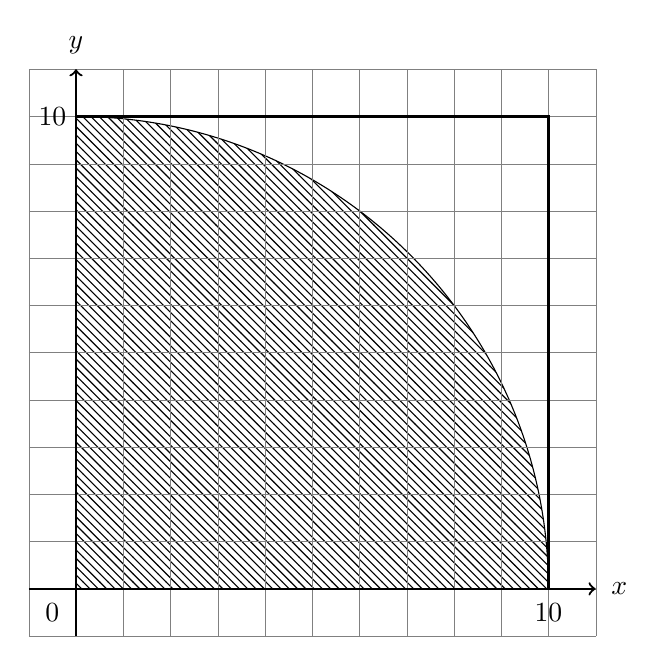
\begin{tikzpicture}[scale=0.6]
			\draw[fill=red!50,pattern=north west lines] (0,0) -- (0,10) arc (90:0:10);
			\draw[ultra thin,gray] (-1,-1) grid (11,11);
			\draw[thick,->] (-1,0) -- (11,0);
			\draw[thick,->] (0,-1) -- (0,11);
			\draw[very thick] (10,0) -- (10,10) -- (0,10);

			\node at (-0.5,-0.5) {$0$};
			\node at (10,-0.5) {$10$};
			\node at (-0.5,10) {$10$};
			\node at (11.5,0) {$x$};
			\node at (0,11.5) {$y$};
		\end{tikzpicture}
	\end{center}
\end{minipage}
\begin{minipage}{0.4\textwidth}
	On considère la figure ci-contre, formée d'un carré de côté $10$cm (non à l'échelle), et d'un quart de cercle de rayon $10$cm.

	On cherche une méthode qui nous permettra de trouver l'aire de la zone hachurée de manière \uline{expérimentale}.
\end{minipage} \bigskip

\begin{enumerate}
	\item Quelle est l'aire du carré ?
	\item Si l'aire de la zone hachurée est appelée $A$, quelle est alors la probabilité qu'un point du carré se trouve dans la zone hachurée ?
	\item On choisit $P$ un point dans le carré de côté $10$, de coordonnées $(x ; y)$.

	      Quelle est la condition sur $x$ et $y$ pour que le point soit dans la zone hachurée ? (Indice : on peut considérer la distance entre $A$ et l'origine)
	\item Compléter la fonction Python ci-dessous, qui détermine si un point du carré est dans la zone hachurée :
	      \begin{lstlisting}
def point_est_dans_zone(x, y):
	return ........ < ........
\end{lstlisting}
	\item On implémente alors la fonction Python suivante, qui simule le choix aléatoire de $N$ points dans le carré, et renvoie la fréquences des points dans la zone hachurée :
	      \begin{lstlisting}
from random import random
def monte_carlo(N):
	pts_dans_zone = 0
	for i in range(N):
		x = 10*random()
		y = 10*random()
		if point_est_dans_zone(x, y):
			pts_dans_zone = pts_dans_zone + 1
	frequence = pts_dans_zone / N
	return frequence
\end{lstlisting}

	      Implémenter et utiliser cette fonction dans une calculatrice pour remplir le tableau suivant :

	      (Alternativement, une simulation sera faite au tableau)

	      \begin{center}
		      \begin{tabular}{|l|*{3}{>{\centering}p{2cm}|}}
			      \hline
			      Nombre de points & $100$ & $1000$ & $10000$ \tabularnewline \hline
			      Fréquence        &       &        & \tabularnewline \hline
		      \end{tabular}
	      \end{center}
	\item En déduire une approximation de l'aire hachurée.
	\item Calculer l'aire exacte de la zone hachurée. Quelle est le pourcentage d'erreur entre cette aire théorique et le résultat de la question précédente ?
\end{enumerate}

\end{document}